% Für Bindekorrektur als optionales Argument "BCORfaktormitmaßeinheit", dann
% sieht auch Option "twoside" vernünftig aus
% Näheres zu "scrartcl" bzw. "scrreprt" und "scrbook" siehe KOMA-Skript Doku
\documentclass[12pt,a4paper,titlepage,headinclude,bibtotoc]{scrartcl}


%---- Allgemeine Layout Einstellungen ------------------------------------------

% Für Kopf und Fußzeilen, siehe auch KOMA-Skript Doku
\usepackage[komastyle]{scrpage2}
\pagestyle{scrheadings}
\automark[section]{chapter}
\setheadsepline{0.5pt}[\color{black}]

%keine Einrückung
\parindent0pt

%Einstellungen für Figuren- und Tabellenbeschriftungen
\setkomafont{captionlabel}{\sffamily\bfseries}
\setcapindent{0em}

\usepackage{caption}
\usepackage{multirow}

%---- Weitere Pakete -----------------------------------------------------------
% Die Pakete sind alle in der TeX Live Distribution enthalten. Wichtige Adressen
% www.ctan.org, www.dante.de

% Sprachunterstützung
\usepackage[ngerman]{babel}

% Benutzung von Umlauten direkt im Text
% entweder "latin1" oder "utf8"
\usepackage[utf8]{inputenc}

% Pakete mit Mathesymbolen und zur Beseitigung von Schwächen der Mathe-Umgebung
\usepackage{latexsym,exscale,amssymb,amsmath}

% Weitere Symbole
\usepackage[nointegrals]{wasysym}
\usepackage{eurosym}

% Anderes Literaturverzeichnisformat
%\usepackage[square,sort&compress]{natbib}

% Für Farbe
\usepackage{color}

% Zur Graphikausgabe
%Beipiel: \includegraphics[width=\textwidth]{grafik.png}
\usepackage{graphicx}

% Text umfließt Graphiken und Tabellen
% Beispiel:
% \begin{wrapfigure}[Zeilenanzahl]{"l" oder "r"}{breite}
%   \centering
%   \includegraphics[width=...]{grafik}
%   \caption{Beschriftung} 
%   \label{fig:grafik}
% \end{wrapfigure}
\usepackage{wrapfig}

% Mehrere Abbildungen nebeneinander
% Beispiel:
% \begin{figure}[htb]
%   \centering
%   \subfigure[Beschriftung 1\label{fig:label1}]
%   {\includegraphics[width=0.49\textwidth]{grafik1}}
%   \hfill
%   \subfigure[Beschriftung 2\label{fig:label2}]
%   {\includegraphics[width=0.49\textwidth]{grafik2}}
%   \caption{Beschriftung allgemein}
%   \label{fig:label-gesamt}
% \end{figure}
\usepackage{subfigure}
\usepackage{adjustbox}

% Caption neben Abbildung
% Beispiel:
% \sidecaptionvpos{figure}{"c" oder "t" oder "b"}
% \begin{SCfigure}[rel. Breite (normalerweise = 1)][hbt]
%   \centering
%   \includegraphics[width=0.5\textwidth]{grafik.png}
%   \caption{Beschreibung}
%   \label{fig:}
% \end{SCfigure}
\usepackage{sidecap}

% Befehl für "Entspricht"-Zeichen
\newcommand{\corresponds}{\ensuremath{\mathrel{\widehat{=}}}}

%Für chemische Formeln (von www.dante.de)
%% Anpassung an LaTeX(2e) von Bernd Raichle
\makeatletter
\DeclareRobustCommand{\chemical}[1]{%
  {\(\m@th
   \edef\resetfontdimens{\noexpand\)%
       \fontdimen16\textfont2=\the\fontdimen16\textfont2
       \fontdimen17\textfont2=\the\fontdimen17\textfont2\relax}%
   \fontdimen16\textfont2=2.7pt \fontdimen17\textfont2=2.7pt
   \mathrm{#1}%
   \resetfontdimens}}
\makeatother

%Si Einheiten
\usepackage{siunitx}

%c++ Code einbinden
\usepackage{listings}
\lstset{numbers=left, numberstyle=\tiny, numbersep=5pt}

%Differential
\newcommand{\dif}{\ensuremath{\mathrm{d}}}

%Boxen,etc.
\usepackage{fancybox}
\usepackage{empheq}

%Fußnoten auf gleiche Seite
\interfootnotelinepenalty=1000

%Dateien aus Unterverzeichnissen
\usepackage{import}

%Bibliography \bibliography{literatur} und \cite{gerthsen}
%\usepackage{cite}
\usepackage{babelbib}
\selectbiblanguage{ngerman}

\begin{document}

\begin{titlepage}
\centering
\textsc{\Large Anfängerpraktikum der Fakultät für
  Physik,\\[1.5ex] Universität Göttingen}

\vspace*{4.2cm}

\rule{\textwidth}{1pt}\\[0.5cm]
{\huge \bfseries
  Versuch 23\\[1.5ex]
  Röntgenstrahlung}\\[0.5cm]
\rule{\textwidth}{1pt}

\vspace*{3.0cm}

\begin{Large}
\begin{tabular}{ll}
Praktikant:
 	&  Felix Kurtz\\
 	&  Michael Lohmann\\

E-Mail: 
	&  felix.kurtz@stud.uni-goettingen.de\\
	& m.lohmann@stud.uni-goettingen.de\\

 Betreuer: & Phillip Bastian\\
 Versuchsdatum: &  11.03.2015\\
\end{tabular}
\end{Large}

\vspace*{0.8cm}

\begin{Large}
\fbox{
  \begin{minipage}[t][2.5cm][t]{6cm} 
    Testat:
  \end{minipage}
}
\end{Large}

\end{titlepage}

\tableofcontents

\newpage

\section{Einleitung}
\label{sec:einleitung}
In diesem Versuch sollen mithilfe der Bragg-Reflexion die Eigenschaften von Röntgenstrahlung untersucht werden.
Dabei kann zum einen die \emph{Bremsstrahlung} als auch die für jedes Material \emph{charakteristische Strahlung} beobachtet werden.
Außerdem werden noch zwei Naturkonstanten der Atomphysik bestimmt: das \emph{Plancksche Wirkungsquantum} und die \emph{Rydberg-Frequenz}.

\section{Theorie}
\label{sec:theorie}
\subsection{Röntgenröhre und Bragg-Reflexion}
In einer Röntgenröhre (vgl. Abb.\ref{fig:Aufbau}) werden Elektronen durch einen Glühdraht emittiert und anschließend auf eine Anode beschleunigt.
Dort wechselwirken sie mit dem Anodenmaterial und es entsteht elektromagnetische Strahlung.
Diese ist bei den typischen Beschleunigungsspannungen $U_A$, die sich bei mehren Kilo-Volt bewegen, energiereicher als Licht.
Man nennt sie im deutschen Sprachraum nach ihrem Entdecker \textsc{Wilhelm Conrad Röntgen} \emph{Röntgenstrahlung}. \\
\begin{figure}[!h]
	\centering
	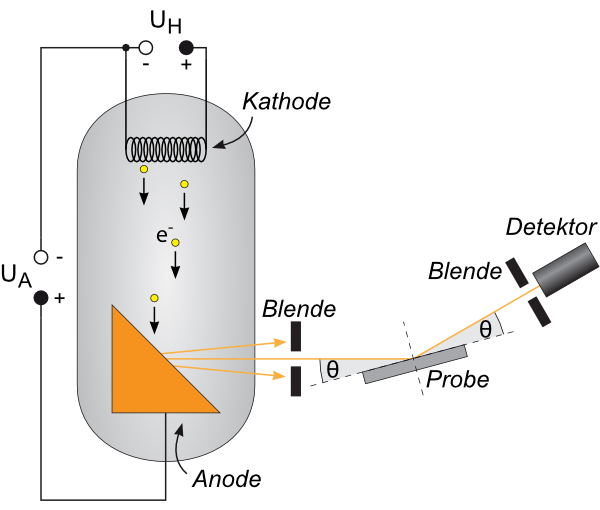
\includegraphics[scale=0.7]{Aufbau.png}
	\caption{Aufbau einer Röntgenröhre mit Detektor. \cite[Datum: 02.01.15]{LP23}}
	\label{fig:Aufbau}
\end{figure}

Um die Strahlung zu charakterisieren, trifft sie auf ein Kristallgitter, dessen Atomabstand im Bereich der Wellenlänge liegt.
Dort kommt es zur \emph{Bragg-Reflexion}, welche in Abb.\ref{fig:Bragg} dargestellt wird.
Die Strahlen werden an mehreren Kristallschichten reflektiert.
Dabei kommt es zu Gangunterschieden, welche ein ganzzahliges Vielfaches $n$ der Wellenlänge sein müssen, damit es zur konstruktiven Interferenz kommt und man am Detektor ein Signal erkennt.
So lässt sich also der Ablenkwinkel $2\theta$ in eine bestimmte Wellenlänge $\lambda$ umrechnen:
\begin{align}
	2d\sin\theta=n\lambda\,.
	\label{eq:Bragg}
\end{align}
Dies nennt man die \emph{Bragg-Bedingung}.

\begin{figure}[!h]
	\centering
	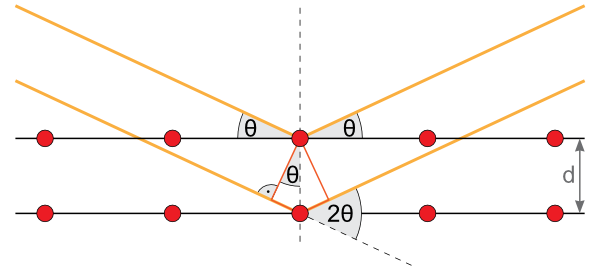
\includegraphics[scale=0.7]{Bragg.png}
	\caption{Bragg-Reflexion schematisch. \cite[Datum: 02.01.15]{LP23}}
	\label{fig:Bragg}
\end{figure}

\subsection{Geiger-Müller-Zählrohr}
Die Röntgenstrahlung wird durch ein Geiger-Müller-Zählrohr detektiert.
Dort ionisiert sie nämlich Atome und setzt somit Elektronen frei.
Diese lösen eine Kaskade an weiteren Elektronen aus und ein Strom kann gemessen werden.
Da das Zählrohr eine gewisse Zeit benötigt, bis es ein neues Ereignis detektieren kann, (\emph{Totzeit}), müssen die Impulsraten $N$ (Impulse/Sekunde) durch folgende Formel korrigiert werden:
\begin{align}
	N_\text{korrigiert}=\frac{N_\text{gemessen}}{1-\tau\cdot N_\text{gemessen}}\,.
\end{align}
Dabei ist $\tau$ die Totzeit, die sich typischerweise im Bereich von $100 ~ \mu$s befindet.
Man berechnet nämlich die Wahrscheinlichkeit mit ein, dass ein Ereignis stattgefunden hat, dieses aber nicht detektiert werden konnte.

\subsection{Bremsstrahlung}
Das Elektron überträgt Energie an das Photon, wenn es mit dem Anodenmaterial wechselwirkt.
Läuft dieser Prozess ideal ab, gibt das Elektron seine gesamte Energie $E=e\cdot U_A$ an das Photon ab, dessen Energie $E=h\cdot \nu=\frac{hc}{\lambda}$ beträgt.
Setzt man also beide Energien gleich, kann man die minimal erreichbare Wellenlänge $\lambda_\text{gr}$ berechnen:
\begin{align}
	\lambda_\text{gr}=\frac{hc}{e \cdot U_A}\,.
	\label{eq:grenzLambda}
\end{align}
Sie hängt nur von der Beschleunigungsspannung $U_A$ ab, da die Elektronenladung $e$, die Vakuum-Lichtgeschwindigkeit $c$ sowie das Plancksche Wirkungsquantum $h$ Naturkonstanten sind.\\
Da aber die wenigsten Photonen die gesamte Elektronenenergie erhalten, ergibt sich eine typische, kontinuierliche Intensitätsverteilung, deren Maximum sich bei einer etwas größeren Wellenlänge befindet.
Man nennt dies \emph{Bremsstrahlung}.

\subsection{Charakteristische Röntgenstrahlung}
Neben der Bremsstrahlung misst man auch noch die für das Anodenmaterial \emph{charakteristische Strahlung}.
Dabei entspricht die Photonen-Energie genau einer Differenz von zwei Energieniveaus: $E_\text{ph}=h\nu=E_s-E_f$.
Ist das untere Niveau $E_f$ die K-Schale, spricht man von K-Linien.
Der Übergang von der L-Schale auf die K-Schale wird mit K$\alpha$ bezeichnet, der von M-Schale mit K$\beta$.
Diese Energiedifferenzen der K-Linien kann man mithilfe des \emph{Moseley-Gesetzes}
\begin{align}
	\nu_K=R_\nu (Z-1)^2\left(\frac{1}{n_f^2}-\frac{1}{n_s^2}\right)
\end{align}
berechnen.
Dabei ist $\nu_K$ die Frequenz des Photons, $R_\nu$ die \emph{Rydberg-Frequenz}, $Z$ die Kernladungszahl des Atoms und $n_s$ bzw. $n_f$ kennzeichnen das obere/untere Niveau.
Für die K-Schale ist $n=1$, für die L-Schale gilt $n=2$, etc.
Analog kann man auch die Energien für die anderen Linien berechnen.
Dabei muss aber die Kernladungszahl um die für jede Schale typische Abschirmkonstante $\sigma$ verringert werden.
Anhand der obigen Formel (K-Schale) erkennt man: $\sigma_K=1$.\\

Die Intensität $I_K$ der charakteristischen Strahlung hängt über
\begin{align}
	I_K \sim I_A\cdot(U_A-U_K)^{3/2}
	\label{eq:IntChara}
\end{align}
von dem Anodenstrom $I_A$ sowie der Anodenspannung $U_A$ und dem Ionisationspotential $U_K$ ab.

\section{Durchführung}
\label{sec:durchfuehrung}
Zuerst wird das Anodenmaterial notiert.
Da wir mit der Eisen-Röhre gearbeitet haben, werden die einzustellenden Werte nur für diese angegeben.\\
Nach Anschalten der Röntgenröhre, des Computers und Starten des Messprogramms \textsc{measure} wird zuerst die charakteristische Strahlung vermessen.
Im Programm stellt man dazu folgende Werte ein: Anodenspannung $U=25\,$kV, Anodenstrom $I=1\,$mA, Winkelschritt $\Delta\theta=0.1^\circ$ und Integrationszeit $\Delta t=2\,$s sowie den zu vermessenden Winkelbereich.
Dieser ist für jedes Anodenmaterial unterschiedlich, für Eisen soll zwischen $\theta_\text{min}=3^\circ$ und $\theta_\text{max}=80^\circ$ gemessen werden.\\
Danach vermisst man für die Spannungen $U=23, 26, 29, 32 \text{ und } 35\,$kV die Grenzwellenlänge und die Intensität der charakteristischen Strahlung, also für Eisen den Winkelbereich zwischen $3^\circ$ und $15^\circ$ sowie zwischen $17^\circ$ und $24^\circ$.
Wieder ist $I=1\,$mA, $\Delta\theta=0.1^\circ$ und $\Delta t=2\,$s.\\
Als nächstes werden die Absorptionskanten von Kupfer und Nickel vermessen.
In der Ablage auf dem Gerät befindet sich ein Kästchen mit Absorptionsfolien.
Man wählt die entsprechenden mit deiner Dicke von 0.025 mm.
Die weiteren Werte betragen $U=25\,$kV, $I=1\,$mA, $\Delta\theta=0.1^\circ$ und $\Delta t=30\,$s.\\
Als letztes wird in einem Bereich zwischen $8^\circ$ und $16^\circ$ mit $\Delta\theta=1^\circ$ die Absorption verschiedener Materialien (verschiedene Kernladungszahlen) vermessen.
Dazu wird als erstes ein Spektrum ohne Absorber aufgenommen, dann 0.08 mm dickes Aluminium sowie 0.025 mm dickes Zink und Zinn.
Die weiteren Werte betragen $U=25\,$kV, $I=1\,$mA und $\Delta t=30\,$s.

\section{Auswertung}
\label{sec:auswertung}
\subsection{Charakteristisches Spektrum von Eisen}
\subsubsection{Wellenlängen und Energien}
\begin{figure}[!htb]
	\centering
	% GNUPLOT: LaTeX picture with Postscript
\begingroup
  \makeatletter
  \providecommand\color[2][]{%
    \GenericError{(gnuplot) \space\space\space\@spaces}{%
      Package color not loaded in conjunction with
      terminal option `colourtext'%
    }{See the gnuplot documentation for explanation.%
    }{Either use 'blacktext' in gnuplot or load the package
      color.sty in LaTeX.}%
    \renewcommand\color[2][]{}%
  }%
  \providecommand\includegraphics[2][]{%
    \GenericError{(gnuplot) \space\space\space\@spaces}{%
      Package graphicx or graphics not loaded%
    }{See the gnuplot documentation for explanation.%
    }{The gnuplot epslatex terminal needs graphicx.sty or graphics.sty.}%
    \renewcommand\includegraphics[2][]{}%
  }%
  \providecommand\rotatebox[2]{#2}%
  \@ifundefined{ifGPcolor}{%
    \newif\ifGPcolor
    \GPcolortrue
  }{}%
  \@ifundefined{ifGPblacktext}{%
    \newif\ifGPblacktext
    \GPblacktexttrue
  }{}%
  % define a \g@addto@macro without @ in the name:
  \let\gplgaddtomacro\g@addto@macro
  % define empty templates for all commands taking text:
  \gdef\gplbacktext{}%
  \gdef\gplfronttext{}%
  \makeatother
  \ifGPblacktext
    % no textcolor at all
    \def\colorrgb#1{}%
    \def\colorgray#1{}%
  \else
    % gray or color?
    \ifGPcolor
      \def\colorrgb#1{\color[rgb]{#1}}%
      \def\colorgray#1{\color[gray]{#1}}%
      \expandafter\def\csname LTw\endcsname{\color{white}}%
      \expandafter\def\csname LTb\endcsname{\color{black}}%
      \expandafter\def\csname LTa\endcsname{\color{black}}%
      \expandafter\def\csname LT0\endcsname{\color[rgb]{1,0,0}}%
      \expandafter\def\csname LT1\endcsname{\color[rgb]{0,1,0}}%
      \expandafter\def\csname LT2\endcsname{\color[rgb]{0,0,1}}%
      \expandafter\def\csname LT3\endcsname{\color[rgb]{1,0,1}}%
      \expandafter\def\csname LT4\endcsname{\color[rgb]{0,1,1}}%
      \expandafter\def\csname LT5\endcsname{\color[rgb]{1,1,0}}%
      \expandafter\def\csname LT6\endcsname{\color[rgb]{0,0,0}}%
      \expandafter\def\csname LT7\endcsname{\color[rgb]{1,0.3,0}}%
      \expandafter\def\csname LT8\endcsname{\color[rgb]{0.5,0.5,0.5}}%
    \else
      % gray
      \def\colorrgb#1{\color{black}}%
      \def\colorgray#1{\color[gray]{#1}}%
      \expandafter\def\csname LTw\endcsname{\color{white}}%
      \expandafter\def\csname LTb\endcsname{\color{black}}%
      \expandafter\def\csname LTa\endcsname{\color{black}}%
      \expandafter\def\csname LT0\endcsname{\color{black}}%
      \expandafter\def\csname LT1\endcsname{\color{black}}%
      \expandafter\def\csname LT2\endcsname{\color{black}}%
      \expandafter\def\csname LT3\endcsname{\color{black}}%
      \expandafter\def\csname LT4\endcsname{\color{black}}%
      \expandafter\def\csname LT5\endcsname{\color{black}}%
      \expandafter\def\csname LT6\endcsname{\color{black}}%
      \expandafter\def\csname LT7\endcsname{\color{black}}%
      \expandafter\def\csname LT8\endcsname{\color{black}}%
    \fi
  \fi
    \setlength{\unitlength}{0.0500bp}%
    \ifx\gptboxheight\undefined%
      \newlength{\gptboxheight}%
      \newlength{\gptboxwidth}%
      \newsavebox{\gptboxtext}%
    \fi%
    \setlength{\fboxrule}{0.5pt}%
    \setlength{\fboxsep}{1pt}%
\begin{picture}(7200.00,5040.00)%
    \gplgaddtomacro\gplbacktext{%
      \csname LTb\endcsname%
      \put(946,704){\makebox(0,0)[r]{\strut{}$0$}}%
      \put(946,1382){\makebox(0,0)[r]{\strut{}$1000$}}%
      \put(946,2061){\makebox(0,0)[r]{\strut{}$2000$}}%
      \put(946,2739){\makebox(0,0)[r]{\strut{}$3000$}}%
      \put(946,3418){\makebox(0,0)[r]{\strut{}$4000$}}%
      \put(946,4096){\makebox(0,0)[r]{\strut{}$5000$}}%
      \put(946,4775){\makebox(0,0)[r]{\strut{}$6000$}}%
      \put(1078,484){\makebox(0,0){\strut{}$0$}}%
      \put(1794,484){\makebox(0,0){\strut{}$10$}}%
      \put(2509,484){\makebox(0,0){\strut{}$20$}}%
      \put(3225,484){\makebox(0,0){\strut{}$30$}}%
      \put(3941,484){\makebox(0,0){\strut{}$40$}}%
      \put(4656,484){\makebox(0,0){\strut{}$50$}}%
      \put(5372,484){\makebox(0,0){\strut{}$60$}}%
      \put(6087,484){\makebox(0,0){\strut{}$70$}}%
      \put(6803,484){\makebox(0,0){\strut{}$80$}}%
    }%
    \gplgaddtomacro\gplfronttext{%
      \csname LTb\endcsname%
      \put(176,2739){\rotatebox{-270}{\makebox(0,0){\strut{}Imp/s}}}%
      \put(3940,154){\makebox(0,0){\strut{}Winkel $\theta$}}%
      \csname LTb\endcsname%
      \put(5816,4602){\makebox(0,0)[r]{\strut{}Messwerte}}%
    }%
    \gplbacktext
    \put(0,0){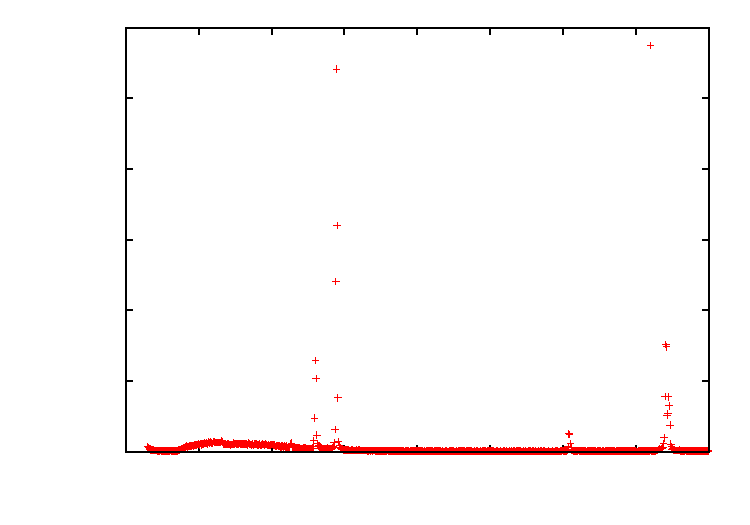
\includegraphics{messung2}}%
    \gplfronttext
  \end{picture}%
\endgroup

	\caption{Spektrum aus Messung 2}
\end{figure}
\begin{table}[!htb]
	\centering
	\begin{tabular}{|c|c|c|c|c|c|}
		\hline
		&&&&\multicolumn{2}{c|}{Energie $E$ [eV]} \\		
		&$n$& Winkel $\theta$ & Wellenlänge $\lambda$ [pm] & Messwert & Lit. Wert\\
		\hline
		\multirow{2}*{K$_{\alpha}$} & 1 & $28.9^\circ \pm 0.2^\circ$ &  $194.3 \pm 1.3$& $6380 \pm 50$ & \multirow{2}*{6391, 6404}  \\
		& 2 & $74.1^\circ \pm 0.2^\circ$ & $193.3 \pm 0.2$ & $6414 \pm 14$  & \\
		\hline
		\multirow{2}*{K$_\beta$} & 1 & $26.0^\circ \pm 0.2^\circ$ & $176.2 \pm 1.3$ & $7040 \pm 60$ & \multirow{2}*{7058} \\
		& 2 & $60.8^\circ \pm 0.2^\circ$ &  $175.5 \pm 0.4$& $7065 \pm 17$ &\\
		\hline
	\end{tabular}
\end{table}

\subsubsection{Abhängigkeit von der Anodenspannung}
\begin{figure}[!htb]
	\centering
	% GNUPLOT: LaTeX picture with Postscript
\begingroup
  \makeatletter
  \providecommand\color[2][]{%
    \GenericError{(gnuplot) \space\space\space\@spaces}{%
      Package color not loaded in conjunction with
      terminal option `colourtext'%
    }{See the gnuplot documentation for explanation.%
    }{Either use 'blacktext' in gnuplot or load the package
      color.sty in LaTeX.}%
    \renewcommand\color[2][]{}%
  }%
  \providecommand\includegraphics[2][]{%
    \GenericError{(gnuplot) \space\space\space\@spaces}{%
      Package graphicx or graphics not loaded%
    }{See the gnuplot documentation for explanation.%
    }{The gnuplot epslatex terminal needs graphicx.sty or graphics.sty.}%
    \renewcommand\includegraphics[2][]{}%
  }%
  \providecommand\rotatebox[2]{#2}%
  \@ifundefined{ifGPcolor}{%
    \newif\ifGPcolor
    \GPcolortrue
  }{}%
  \@ifundefined{ifGPblacktext}{%
    \newif\ifGPblacktext
    \GPblacktexttrue
  }{}%
  % define a \g@addto@macro without @ in the name:
  \let\gplgaddtomacro\g@addto@macro
  % define empty templates for all commands taking text:
  \gdef\gplbacktext{}%
  \gdef\gplfronttext{}%
  \makeatother
  \ifGPblacktext
    % no textcolor at all
    \def\colorrgb#1{}%
    \def\colorgray#1{}%
  \else
    % gray or color?
    \ifGPcolor
      \def\colorrgb#1{\color[rgb]{#1}}%
      \def\colorgray#1{\color[gray]{#1}}%
      \expandafter\def\csname LTw\endcsname{\color{white}}%
      \expandafter\def\csname LTb\endcsname{\color{black}}%
      \expandafter\def\csname LTa\endcsname{\color{black}}%
      \expandafter\def\csname LT0\endcsname{\color[rgb]{1,0,0}}%
      \expandafter\def\csname LT1\endcsname{\color[rgb]{0,1,0}}%
      \expandafter\def\csname LT2\endcsname{\color[rgb]{0,0,1}}%
      \expandafter\def\csname LT3\endcsname{\color[rgb]{1,0,1}}%
      \expandafter\def\csname LT4\endcsname{\color[rgb]{0,1,1}}%
      \expandafter\def\csname LT5\endcsname{\color[rgb]{1,1,0}}%
      \expandafter\def\csname LT6\endcsname{\color[rgb]{0,0,0}}%
      \expandafter\def\csname LT7\endcsname{\color[rgb]{1,0.3,0}}%
      \expandafter\def\csname LT8\endcsname{\color[rgb]{0.5,0.5,0.5}}%
    \else
      % gray
      \def\colorrgb#1{\color{black}}%
      \def\colorgray#1{\color[gray]{#1}}%
      \expandafter\def\csname LTw\endcsname{\color{white}}%
      \expandafter\def\csname LTb\endcsname{\color{black}}%
      \expandafter\def\csname LTa\endcsname{\color{black}}%
      \expandafter\def\csname LT0\endcsname{\color{black}}%
      \expandafter\def\csname LT1\endcsname{\color{black}}%
      \expandafter\def\csname LT2\endcsname{\color{black}}%
      \expandafter\def\csname LT3\endcsname{\color{black}}%
      \expandafter\def\csname LT4\endcsname{\color{black}}%
      \expandafter\def\csname LT5\endcsname{\color{black}}%
      \expandafter\def\csname LT6\endcsname{\color{black}}%
      \expandafter\def\csname LT7\endcsname{\color{black}}%
      \expandafter\def\csname LT8\endcsname{\color{black}}%
    \fi
  \fi
  \setlength{\unitlength}{0.0500bp}%
  \begin{picture}(7200.00,5040.00)%
    \gplgaddtomacro\gplbacktext{%
      \csname LTb\endcsname%
      \put(1210,704){\makebox(0,0)[r]{\strut{} 0}}%
      \put(1210,1213){\makebox(0,0)[r]{\strut{} 2000}}%
      \put(1210,1722){\makebox(0,0)[r]{\strut{} 4000}}%
      \put(1210,2231){\makebox(0,0)[r]{\strut{} 6000}}%
      \put(1210,2740){\makebox(0,0)[r]{\strut{} 8000}}%
      \put(1210,3248){\makebox(0,0)[r]{\strut{} 10000}}%
      \put(1210,3757){\makebox(0,0)[r]{\strut{} 12000}}%
      \put(1210,4266){\makebox(0,0)[r]{\strut{} 14000}}%
      \put(1210,4775){\makebox(0,0)[r]{\strut{} 16000}}%
      \put(1342,484){\makebox(0,0){\strut{} 24}}%
      \put(2122,484){\makebox(0,0){\strut{} 25}}%
      \put(2902,484){\makebox(0,0){\strut{} 26}}%
      \put(3682,484){\makebox(0,0){\strut{} 27}}%
      \put(4463,484){\makebox(0,0){\strut{} 28}}%
      \put(5243,484){\makebox(0,0){\strut{} 29}}%
      \put(6023,484){\makebox(0,0){\strut{} 30}}%
      \put(6803,484){\makebox(0,0){\strut{} 31}}%
      \put(176,2739){\rotatebox{-270}{\makebox(0,0){\strut{}Imp/s}}}%
      \put(4072,154){\makebox(0,0){\strut{}Kristallwinkel $\theta$}}%
    }%
    \gplgaddtomacro\gplfronttext{%
      \csname LTb\endcsname%
      \put(2662,4602){\makebox(0,0)[r]{\strut{}$U_A=23\,$kV}}%
      \csname LTb\endcsname%
      \put(2662,4382){\makebox(0,0)[r]{\strut{}$U_A=26\,$kV}}%
      \csname LTb\endcsname%
      \put(2662,4162){\makebox(0,0)[r]{\strut{}$U_A=29\,$kV}}%
      \csname LTb\endcsname%
      \put(2662,3942){\makebox(0,0)[r]{\strut{}$U_A=32\,$kV}}%
      \csname LTb\endcsname%
      \put(2662,3722){\makebox(0,0)[r]{\strut{}$U_A=35\,$kV}}%
    }%
    \gplbacktext
    \put(0,0){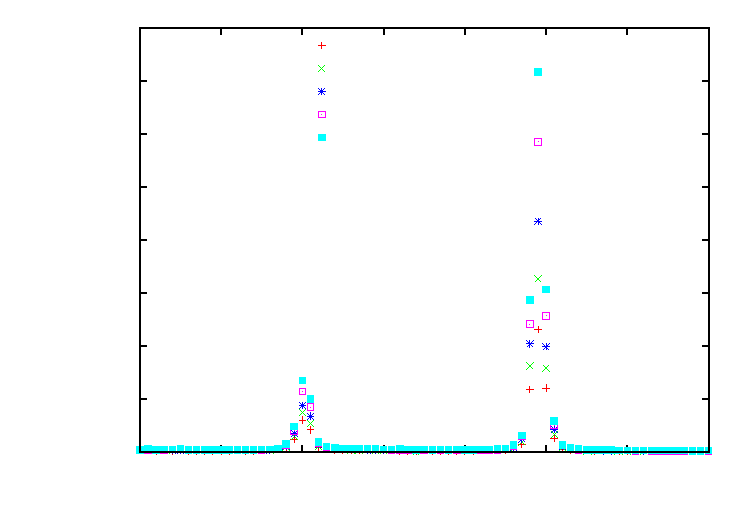
\includegraphics{messung3b}}%
    \gplfronttext
  \end{picture}%
\endgroup

	\caption{Messwerte im Bereich der charakteristischen Strahlung}
\end{figure}

\begin{figure}
	\centering
	% GNUPLOT: LaTeX picture with Postscript
\begingroup
  \makeatletter
  \providecommand\color[2][]{%
    \GenericError{(gnuplot) \space\space\space\@spaces}{%
      Package color not loaded in conjunction with
      terminal option `colourtext'%
    }{See the gnuplot documentation for explanation.%
    }{Either use 'blacktext' in gnuplot or load the package
      color.sty in LaTeX.}%
    \renewcommand\color[2][]{}%
  }%
  \providecommand\includegraphics[2][]{%
    \GenericError{(gnuplot) \space\space\space\@spaces}{%
      Package graphicx or graphics not loaded%
    }{See the gnuplot documentation for explanation.%
    }{The gnuplot epslatex terminal needs graphicx.sty or graphics.sty.}%
    \renewcommand\includegraphics[2][]{}%
  }%
  \providecommand\rotatebox[2]{#2}%
  \@ifundefined{ifGPcolor}{%
    \newif\ifGPcolor
    \GPcolortrue
  }{}%
  \@ifundefined{ifGPblacktext}{%
    \newif\ifGPblacktext
    \GPblacktexttrue
  }{}%
  % define a \g@addto@macro without @ in the name:
  \let\gplgaddtomacro\g@addto@macro
  % define empty templates for all commands taking text:
  \gdef\gplbacktext{}%
  \gdef\gplfronttext{}%
  \makeatother
  \ifGPblacktext
    % no textcolor at all
    \def\colorrgb#1{}%
    \def\colorgray#1{}%
  \else
    % gray or color?
    \ifGPcolor
      \def\colorrgb#1{\color[rgb]{#1}}%
      \def\colorgray#1{\color[gray]{#1}}%
      \expandafter\def\csname LTw\endcsname{\color{white}}%
      \expandafter\def\csname LTb\endcsname{\color{black}}%
      \expandafter\def\csname LTa\endcsname{\color{black}}%
      \expandafter\def\csname LT0\endcsname{\color[rgb]{1,0,0}}%
      \expandafter\def\csname LT1\endcsname{\color[rgb]{0,1,0}}%
      \expandafter\def\csname LT2\endcsname{\color[rgb]{0,0,1}}%
      \expandafter\def\csname LT3\endcsname{\color[rgb]{1,0,1}}%
      \expandafter\def\csname LT4\endcsname{\color[rgb]{0,1,1}}%
      \expandafter\def\csname LT5\endcsname{\color[rgb]{1,1,0}}%
      \expandafter\def\csname LT6\endcsname{\color[rgb]{0,0,0}}%
      \expandafter\def\csname LT7\endcsname{\color[rgb]{1,0.3,0}}%
      \expandafter\def\csname LT8\endcsname{\color[rgb]{0.5,0.5,0.5}}%
    \else
      % gray
      \def\colorrgb#1{\color{black}}%
      \def\colorgray#1{\color[gray]{#1}}%
      \expandafter\def\csname LTw\endcsname{\color{white}}%
      \expandafter\def\csname LTb\endcsname{\color{black}}%
      \expandafter\def\csname LTa\endcsname{\color{black}}%
      \expandafter\def\csname LT0\endcsname{\color{black}}%
      \expandafter\def\csname LT1\endcsname{\color{black}}%
      \expandafter\def\csname LT2\endcsname{\color{black}}%
      \expandafter\def\csname LT3\endcsname{\color{black}}%
      \expandafter\def\csname LT4\endcsname{\color{black}}%
      \expandafter\def\csname LT5\endcsname{\color{black}}%
      \expandafter\def\csname LT6\endcsname{\color{black}}%
      \expandafter\def\csname LT7\endcsname{\color{black}}%
      \expandafter\def\csname LT8\endcsname{\color{black}}%
    \fi
  \fi
  \setlength{\unitlength}{0.0500bp}%
  \begin{picture}(7200.00,5040.00)%
    \gplgaddtomacro\gplbacktext{%
      \csname LTb\endcsname%
      \put(1210,704){\makebox(0,0)[r]{\strut{} 0}}%
      \put(1210,1213){\makebox(0,0)[r]{\strut{} 2000}}%
      \put(1210,1722){\makebox(0,0)[r]{\strut{} 4000}}%
      \put(1210,2231){\makebox(0,0)[r]{\strut{} 6000}}%
      \put(1210,2740){\makebox(0,0)[r]{\strut{} 8000}}%
      \put(1210,3248){\makebox(0,0)[r]{\strut{} 10000}}%
      \put(1210,3757){\makebox(0,0)[r]{\strut{} 12000}}%
      \put(1210,4266){\makebox(0,0)[r]{\strut{} 14000}}%
      \put(1210,4775){\makebox(0,0)[r]{\strut{} 16000}}%
      \put(1342,484){\makebox(0,0){\strut{} 60}}%
      \put(1888,484){\makebox(0,0){\strut{} 70}}%
      \put(2434,484){\makebox(0,0){\strut{} 80}}%
      \put(2980,484){\makebox(0,0){\strut{} 90}}%
      \put(3526,484){\makebox(0,0){\strut{} 100}}%
      \put(4073,484){\makebox(0,0){\strut{} 110}}%
      \put(4619,484){\makebox(0,0){\strut{} 120}}%
      \put(5165,484){\makebox(0,0){\strut{} 130}}%
      \put(5711,484){\makebox(0,0){\strut{} 140}}%
      \put(6257,484){\makebox(0,0){\strut{} 150}}%
      \put(6803,484){\makebox(0,0){\strut{} 160}}%
      \put(176,2739){\rotatebox{-270}{\makebox(0,0){\strut{}Imp/s}}}%
      \put(4072,154){\makebox(0,0){\strut{}$(U_A-U_K)^{1.5}$}}%
    }%
    \gplgaddtomacro\gplfronttext{%
      \csname LTb\endcsname%
      \put(3058,4602){\makebox(0,0)[r]{\strut{}Messwerte K$_\beta$}}%
      \csname LTb\endcsname%
      \put(3058,4382){\makebox(0,0)[r]{\strut{}Messwerte K$_\alpha$}}%
    }%
    \gplbacktext
    \put(0,0){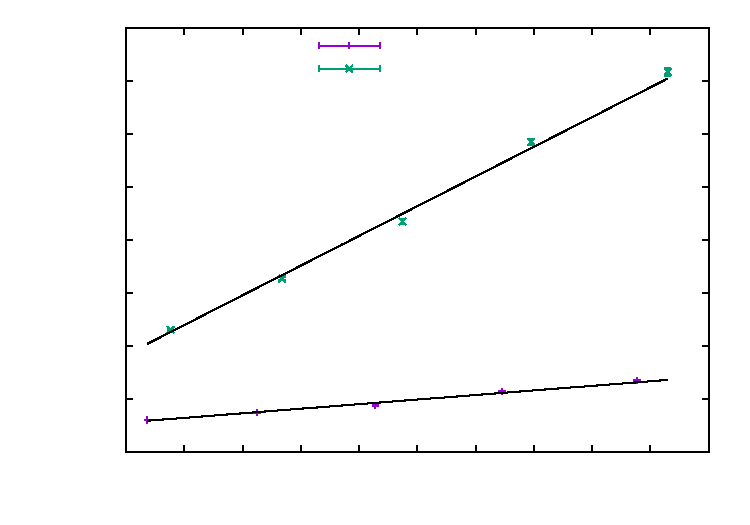
\includegraphics{anode}}%
    \gplfronttext
  \end{picture}%
\endgroup

	\caption{Charakteristische Strahlung: Intensität in Abhängigkeit der Anodenspannnung}
\end{figure}

\subsubsection{Grenzwellenlänge der Bremsstrahlung und Plancksche Konstante}
\begin{figure}[!htb]
	\centering
	% GNUPLOT: LaTeX picture with Postscript
\begingroup
  \makeatletter
  \providecommand\color[2][]{%
    \GenericError{(gnuplot) \space\space\space\@spaces}{%
      Package color not loaded in conjunction with
      terminal option `colourtext'%
    }{See the gnuplot documentation for explanation.%
    }{Either use 'blacktext' in gnuplot or load the package
      color.sty in LaTeX.}%
    \renewcommand\color[2][]{}%
  }%
  \providecommand\includegraphics[2][]{%
    \GenericError{(gnuplot) \space\space\space\@spaces}{%
      Package graphicx or graphics not loaded%
    }{See the gnuplot documentation for explanation.%
    }{The gnuplot epslatex terminal needs graphicx.sty or graphics.sty.}%
    \renewcommand\includegraphics[2][]{}%
  }%
  \providecommand\rotatebox[2]{#2}%
  \@ifundefined{ifGPcolor}{%
    \newif\ifGPcolor
    \GPcolortrue
  }{}%
  \@ifundefined{ifGPblacktext}{%
    \newif\ifGPblacktext
    \GPblacktexttrue
  }{}%
  % define a \g@addto@macro without @ in the name:
  \let\gplgaddtomacro\g@addto@macro
  % define empty templates for all commands taking text:
  \gdef\gplbacktext{}%
  \gdef\gplfronttext{}%
  \makeatother
  \ifGPblacktext
    % no textcolor at all
    \def\colorrgb#1{}%
    \def\colorgray#1{}%
  \else
    % gray or color?
    \ifGPcolor
      \def\colorrgb#1{\color[rgb]{#1}}%
      \def\colorgray#1{\color[gray]{#1}}%
      \expandafter\def\csname LTw\endcsname{\color{white}}%
      \expandafter\def\csname LTb\endcsname{\color{black}}%
      \expandafter\def\csname LTa\endcsname{\color{black}}%
      \expandafter\def\csname LT0\endcsname{\color[rgb]{1,0,0}}%
      \expandafter\def\csname LT1\endcsname{\color[rgb]{0,1,0}}%
      \expandafter\def\csname LT2\endcsname{\color[rgb]{0,0,1}}%
      \expandafter\def\csname LT3\endcsname{\color[rgb]{1,0,1}}%
      \expandafter\def\csname LT4\endcsname{\color[rgb]{0,1,1}}%
      \expandafter\def\csname LT5\endcsname{\color[rgb]{1,1,0}}%
      \expandafter\def\csname LT6\endcsname{\color[rgb]{0,0,0}}%
      \expandafter\def\csname LT7\endcsname{\color[rgb]{1,0.3,0}}%
      \expandafter\def\csname LT8\endcsname{\color[rgb]{0.5,0.5,0.5}}%
    \else
      % gray
      \def\colorrgb#1{\color{black}}%
      \def\colorgray#1{\color[gray]{#1}}%
      \expandafter\def\csname LTw\endcsname{\color{white}}%
      \expandafter\def\csname LTb\endcsname{\color{black}}%
      \expandafter\def\csname LTa\endcsname{\color{black}}%
      \expandafter\def\csname LT0\endcsname{\color{black}}%
      \expandafter\def\csname LT1\endcsname{\color{black}}%
      \expandafter\def\csname LT2\endcsname{\color{black}}%
      \expandafter\def\csname LT3\endcsname{\color{black}}%
      \expandafter\def\csname LT4\endcsname{\color{black}}%
      \expandafter\def\csname LT5\endcsname{\color{black}}%
      \expandafter\def\csname LT6\endcsname{\color{black}}%
      \expandafter\def\csname LT7\endcsname{\color{black}}%
      \expandafter\def\csname LT8\endcsname{\color{black}}%
    \fi
  \fi
  \setlength{\unitlength}{0.0500bp}%
  \begin{picture}(7200.00,5040.00)%
    \gplgaddtomacro\gplbacktext{%
      \csname LTb\endcsname%
      \put(946,704){\makebox(0,0)[r]{\strut{} 0}}%
      \put(946,1213){\makebox(0,0)[r]{\strut{} 50}}%
      \put(946,1722){\makebox(0,0)[r]{\strut{} 100}}%
      \put(946,2231){\makebox(0,0)[r]{\strut{} 150}}%
      \put(946,2740){\makebox(0,0)[r]{\strut{} 200}}%
      \put(946,3248){\makebox(0,0)[r]{\strut{} 250}}%
      \put(946,3757){\makebox(0,0)[r]{\strut{} 300}}%
      \put(946,4266){\makebox(0,0)[r]{\strut{} 350}}%
      \put(946,4775){\makebox(0,0)[r]{\strut{} 400}}%
      \put(1078,484){\makebox(0,0){\strut{} 2}}%
      \put(1896,484){\makebox(0,0){\strut{} 4}}%
      \put(2714,484){\makebox(0,0){\strut{} 6}}%
      \put(3532,484){\makebox(0,0){\strut{} 8}}%
      \put(4349,484){\makebox(0,0){\strut{} 10}}%
      \put(5167,484){\makebox(0,0){\strut{} 12}}%
      \put(5985,484){\makebox(0,0){\strut{} 14}}%
      \put(6803,484){\makebox(0,0){\strut{} 16}}%
      \put(176,2739){\rotatebox{-270}{\makebox(0,0){\strut{}Imp/s}}}%
      \put(3940,154){\makebox(0,0){\strut{}Kristallwinkel $\theta$}}%
    }%
    \gplgaddtomacro\gplfronttext{%
      \csname LTb\endcsname%
      \put(4107,4602){\makebox(0,0)[r]{\strut{}$U_A=23\,$kV}}%
      \csname LTb\endcsname%
      \put(4107,4382){\makebox(0,0)[r]{\strut{}$U_A=26\,$kV}}%
      \csname LTb\endcsname%
      \put(4107,4162){\makebox(0,0)[r]{\strut{}$U_A=29\,$kV}}%
      \csname LTb\endcsname%
      \put(4107,3942){\makebox(0,0)[r]{\strut{}$U_A=32\,$kV}}%
      \csname LTb\endcsname%
      \put(4107,3722){\makebox(0,0)[r]{\strut{}$U_A=35\,$kV}}%
    }%
    \gplbacktext
    \put(0,0){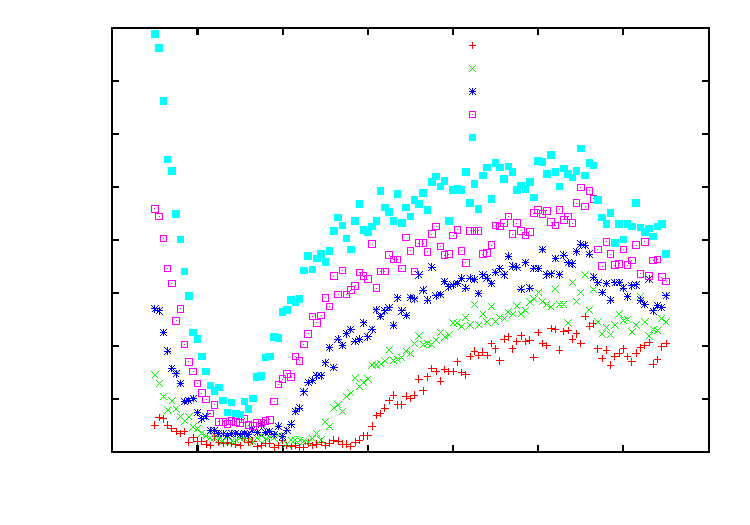
\includegraphics{messung3a}}%
    \gplfronttext
  \end{picture}%
\endgroup

	\caption{Messwerte im Bereich der Grenzwellenlänge}
\end{figure}

\begin{figure}[!htb]
	\centering
	% GNUPLOT: LaTeX picture with Postscript
\begingroup
  \makeatletter
  \providecommand\color[2][]{%
    \GenericError{(gnuplot) \space\space\space\@spaces}{%
      Package color not loaded in conjunction with
      terminal option `colourtext'%
    }{See the gnuplot documentation for explanation.%
    }{Either use 'blacktext' in gnuplot or load the package
      color.sty in LaTeX.}%
    \renewcommand\color[2][]{}%
  }%
  \providecommand\includegraphics[2][]{%
    \GenericError{(gnuplot) \space\space\space\@spaces}{%
      Package graphicx or graphics not loaded%
    }{See the gnuplot documentation for explanation.%
    }{The gnuplot epslatex terminal needs graphicx.sty or graphics.sty.}%
    \renewcommand\includegraphics[2][]{}%
  }%
  \providecommand\rotatebox[2]{#2}%
  \@ifundefined{ifGPcolor}{%
    \newif\ifGPcolor
    \GPcolortrue
  }{}%
  \@ifundefined{ifGPblacktext}{%
    \newif\ifGPblacktext
    \GPblacktexttrue
  }{}%
  % define a \g@addto@macro without @ in the name:
  \let\gplgaddtomacro\g@addto@macro
  % define empty templates for all commands taking text:
  \gdef\gplbacktext{}%
  \gdef\gplfronttext{}%
  \makeatother
  \ifGPblacktext
    % no textcolor at all
    \def\colorrgb#1{}%
    \def\colorgray#1{}%
  \else
    % gray or color?
    \ifGPcolor
      \def\colorrgb#1{\color[rgb]{#1}}%
      \def\colorgray#1{\color[gray]{#1}}%
      \expandafter\def\csname LTw\endcsname{\color{white}}%
      \expandafter\def\csname LTb\endcsname{\color{black}}%
      \expandafter\def\csname LTa\endcsname{\color{black}}%
      \expandafter\def\csname LT0\endcsname{\color[rgb]{1,0,0}}%
      \expandafter\def\csname LT1\endcsname{\color[rgb]{0,1,0}}%
      \expandafter\def\csname LT2\endcsname{\color[rgb]{0,0,1}}%
      \expandafter\def\csname LT3\endcsname{\color[rgb]{1,0,1}}%
      \expandafter\def\csname LT4\endcsname{\color[rgb]{0,1,1}}%
      \expandafter\def\csname LT5\endcsname{\color[rgb]{1,1,0}}%
      \expandafter\def\csname LT6\endcsname{\color[rgb]{0,0,0}}%
      \expandafter\def\csname LT7\endcsname{\color[rgb]{1,0.3,0}}%
      \expandafter\def\csname LT8\endcsname{\color[rgb]{0.5,0.5,0.5}}%
    \else
      % gray
      \def\colorrgb#1{\color{black}}%
      \def\colorgray#1{\color[gray]{#1}}%
      \expandafter\def\csname LTw\endcsname{\color{white}}%
      \expandafter\def\csname LTb\endcsname{\color{black}}%
      \expandafter\def\csname LTa\endcsname{\color{black}}%
      \expandafter\def\csname LT0\endcsname{\color{black}}%
      \expandafter\def\csname LT1\endcsname{\color{black}}%
      \expandafter\def\csname LT2\endcsname{\color{black}}%
      \expandafter\def\csname LT3\endcsname{\color{black}}%
      \expandafter\def\csname LT4\endcsname{\color{black}}%
      \expandafter\def\csname LT5\endcsname{\color{black}}%
      \expandafter\def\csname LT6\endcsname{\color{black}}%
      \expandafter\def\csname LT7\endcsname{\color{black}}%
      \expandafter\def\csname LT8\endcsname{\color{black}}%
    \fi
  \fi
    \setlength{\unitlength}{0.0500bp}%
    \ifx\gptboxheight\undefined%
      \newlength{\gptboxheight}%
      \newlength{\gptboxwidth}%
      \newsavebox{\gptboxtext}%
    \fi%
    \setlength{\fboxrule}{0.5pt}%
    \setlength{\fboxsep}{1pt}%
\begin{picture}(7200.00,5040.00)%
    \gplgaddtomacro\gplbacktext{%
      \csname LTb\endcsname%
      \put(946,704){\makebox(0,0)[r]{\strut{}$1.16$}}%
      \put(946,1286){\makebox(0,0)[r]{\strut{}$1.18$}}%
      \put(946,1867){\makebox(0,0)[r]{\strut{}$1.2$}}%
      \put(946,2449){\makebox(0,0)[r]{\strut{}$1.22$}}%
      \put(946,3030){\makebox(0,0)[r]{\strut{}$1.24$}}%
      \put(946,3612){\makebox(0,0)[r]{\strut{}$1.26$}}%
      \put(946,4193){\makebox(0,0)[r]{\strut{}$1.28$}}%
      \put(946,4775){\makebox(0,0)[r]{\strut{}$1.3$}}%
      \put(1078,484){\makebox(0,0){\strut{}$22$}}%
      \put(1896,484){\makebox(0,0){\strut{}$24$}}%
      \put(2714,484){\makebox(0,0){\strut{}$26$}}%
      \put(3532,484){\makebox(0,0){\strut{}$28$}}%
      \put(4349,484){\makebox(0,0){\strut{}$30$}}%
      \put(5167,484){\makebox(0,0){\strut{}$32$}}%
      \put(5985,484){\makebox(0,0){\strut{}$34$}}%
      \put(6803,484){\makebox(0,0){\strut{}$36$}}%
    }%
    \gplgaddtomacro\gplfronttext{%
      \csname LTb\endcsname%
      \put(176,2739){\rotatebox{-270}{\makebox(0,0){\strut{}$\lambda_\text{gr}\cdot U_A$ [$10^{-6}~$Vm]}}}%
      \put(3940,154){\makebox(0,0){\strut{}Spannung $U_A$ [kV]}}%
      \csname LTb\endcsname%
      \put(5816,4602){\makebox(0,0)[r]{\strut{}Messwerte}}%
      \csname LTb\endcsname%
      \put(5816,4382){\makebox(0,0)[r]{\strut{}Mittelwert}}%
    }%
    \gplbacktext
    \put(0,0){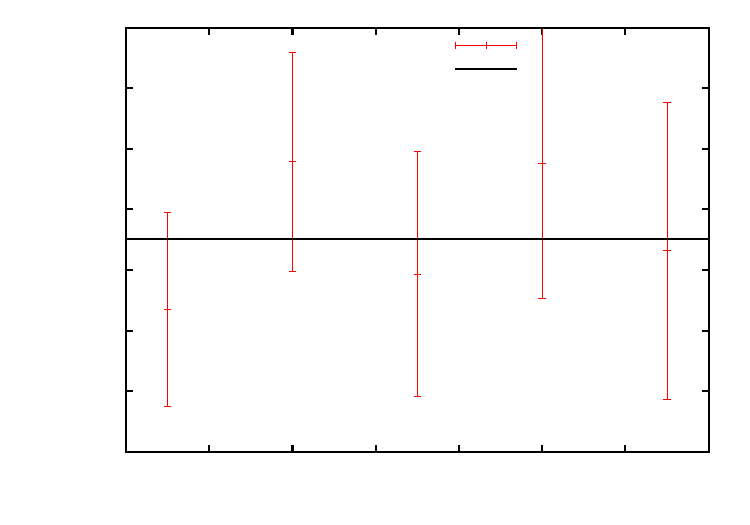
\includegraphics{grenzLambda}}%
    \gplfronttext
  \end{picture}%
\endgroup

	\caption{Produkt aus Beschleunigungsspannung und zugehöriger Grenzwellenlänge in Abhängigkeit der Spannung}
\end{figure}

\begin{empheq}[box=\shadowbox]{align}
	h=(6.57 \pm 0.06)~10^{-34}\si{\joule\second}
\end{empheq}

\subsection{Absorptionskanten und Rydberg-Konstante}
\begin{figure}[!htb]
	\centering
	% GNUPLOT: LaTeX picture with Postscript
\begingroup
  \makeatletter
  \providecommand\color[2][]{%
    \GenericError{(gnuplot) \space\space\space\@spaces}{%
      Package color not loaded in conjunction with
      terminal option `colourtext'%
    }{See the gnuplot documentation for explanation.%
    }{Either use 'blacktext' in gnuplot or load the package
      color.sty in LaTeX.}%
    \renewcommand\color[2][]{}%
  }%
  \providecommand\includegraphics[2][]{%
    \GenericError{(gnuplot) \space\space\space\@spaces}{%
      Package graphicx or graphics not loaded%
    }{See the gnuplot documentation for explanation.%
    }{The gnuplot epslatex terminal needs graphicx.sty or graphics.sty.}%
    \renewcommand\includegraphics[2][]{}%
  }%
  \providecommand\rotatebox[2]{#2}%
  \@ifundefined{ifGPcolor}{%
    \newif\ifGPcolor
    \GPcolortrue
  }{}%
  \@ifundefined{ifGPblacktext}{%
    \newif\ifGPblacktext
    \GPblacktexttrue
  }{}%
  % define a \g@addto@macro without @ in the name:
  \let\gplgaddtomacro\g@addto@macro
  % define empty templates for all commands taking text:
  \gdef\gplbacktext{}%
  \gdef\gplfronttext{}%
  \makeatother
  \ifGPblacktext
    % no textcolor at all
    \def\colorrgb#1{}%
    \def\colorgray#1{}%
  \else
    % gray or color?
    \ifGPcolor
      \def\colorrgb#1{\color[rgb]{#1}}%
      \def\colorgray#1{\color[gray]{#1}}%
      \expandafter\def\csname LTw\endcsname{\color{white}}%
      \expandafter\def\csname LTb\endcsname{\color{black}}%
      \expandafter\def\csname LTa\endcsname{\color{black}}%
      \expandafter\def\csname LT0\endcsname{\color[rgb]{1,0,0}}%
      \expandafter\def\csname LT1\endcsname{\color[rgb]{0,1,0}}%
      \expandafter\def\csname LT2\endcsname{\color[rgb]{0,0,1}}%
      \expandafter\def\csname LT3\endcsname{\color[rgb]{1,0,1}}%
      \expandafter\def\csname LT4\endcsname{\color[rgb]{0,1,1}}%
      \expandafter\def\csname LT5\endcsname{\color[rgb]{1,1,0}}%
      \expandafter\def\csname LT6\endcsname{\color[rgb]{0,0,0}}%
      \expandafter\def\csname LT7\endcsname{\color[rgb]{1,0.3,0}}%
      \expandafter\def\csname LT8\endcsname{\color[rgb]{0.5,0.5,0.5}}%
    \else
      % gray
      \def\colorrgb#1{\color{black}}%
      \def\colorgray#1{\color[gray]{#1}}%
      \expandafter\def\csname LTw\endcsname{\color{white}}%
      \expandafter\def\csname LTb\endcsname{\color{black}}%
      \expandafter\def\csname LTa\endcsname{\color{black}}%
      \expandafter\def\csname LT0\endcsname{\color{black}}%
      \expandafter\def\csname LT1\endcsname{\color{black}}%
      \expandafter\def\csname LT2\endcsname{\color{black}}%
      \expandafter\def\csname LT3\endcsname{\color{black}}%
      \expandafter\def\csname LT4\endcsname{\color{black}}%
      \expandafter\def\csname LT5\endcsname{\color{black}}%
      \expandafter\def\csname LT6\endcsname{\color{black}}%
      \expandafter\def\csname LT7\endcsname{\color{black}}%
      \expandafter\def\csname LT8\endcsname{\color{black}}%
    \fi
  \fi
  \setlength{\unitlength}{0.0500bp}%
  \begin{picture}(7200.00,5040.00)%
    \gplgaddtomacro\gplbacktext{%
      \csname LTb\endcsname%
      \put(946,704){\makebox(0,0)[r]{\strut{} 1}}%
      \put(946,1383){\makebox(0,0)[r]{\strut{} 1.5}}%
      \put(946,2061){\makebox(0,0)[r]{\strut{} 2}}%
      \put(946,2740){\makebox(0,0)[r]{\strut{} 2.5}}%
      \put(946,3418){\makebox(0,0)[r]{\strut{} 3}}%
      \put(946,4097){\makebox(0,0)[r]{\strut{} 3.5}}%
      \put(946,4775){\makebox(0,0)[r]{\strut{} 4}}%
      \put(1078,484){\makebox(0,0){\strut{} 19.5}}%
      \put(1896,484){\makebox(0,0){\strut{} 20}}%
      \put(2714,484){\makebox(0,0){\strut{} 20.5}}%
      \put(3532,484){\makebox(0,0){\strut{} 21}}%
      \put(4349,484){\makebox(0,0){\strut{} 21.5}}%
      \put(5167,484){\makebox(0,0){\strut{} 22}}%
      \put(5985,484){\makebox(0,0){\strut{} 22.5}}%
      \put(6803,484){\makebox(0,0){\strut{} 23}}%
      \put(176,2739){\rotatebox{-270}{\makebox(0,0){\strut{}ln(Imp/s)}}}%
      \put(3940,154){\makebox(0,0){\strut{}Kristallwinkel $\theta$}}%
    }%
    \gplgaddtomacro\gplfronttext{%
      \csname LTb\endcsname%
      \put(5816,4602){\makebox(0,0)[r]{\strut{}Kupfer}}%
      \csname LTb\endcsname%
      \put(5816,4382){\makebox(0,0)[r]{\strut{}Nickel}}%
    }%
    \gplbacktext
    \put(0,0){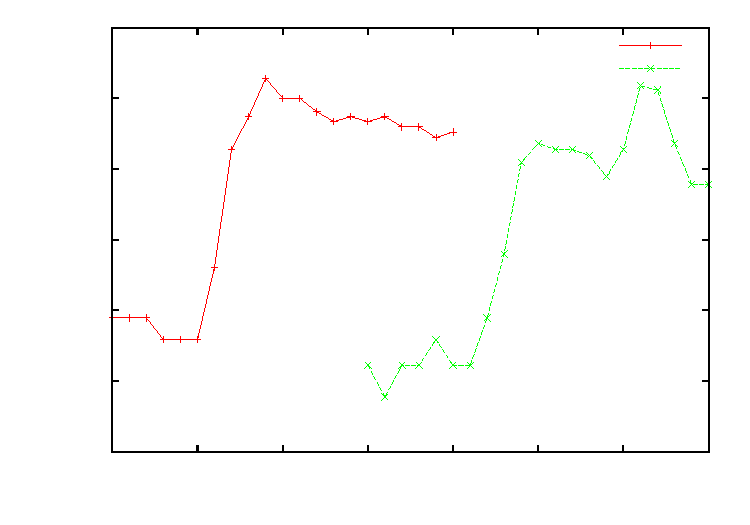
\includegraphics{messung4}}%
    \gplfronttext
  \end{picture}%
\endgroup

	\caption{Absorptionskanten von Kupfer und Nickel: Intensität logarithmisch gegen Winkel aufgetragen}
\end{figure}
\begin{table}
	\centering
	\begin{tabular}{|c|c|c|c|}
		\hline
		& Winkel $\theta$ & Wellenlänge $\lambda$ [pm] & Rydbergfrequenz $R_\nu$\\
		\hline
		Kupfer & $20.2^\circ \pm 0.2^\circ$ & $138.8 \pm 1.4$ & $(3.67 \pm 0.04)\cdot 10^{15}~\si{Hz}$  \\
		Nickel & $21.8^\circ \pm 0.2^\circ$ & $149.8 \pm 1.4$ & $(3.67 \pm 0.04)\cdot 10^{15}~\si{Hz}$  \\
		\hline
	\end{tabular}
	\caption{Absorptionskanten von Kupfer und Nickel und die daraus berechnete Rydbergfrequenz}
\end{table}

\subsection{Absorptionskoeffizienten verschiedener Metalle}
\begin{figure}[!htb]
	\centering
	% GNUPLOT: LaTeX picture with Postscript
\begingroup
  \makeatletter
  \providecommand\color[2][]{%
    \GenericError{(gnuplot) \space\space\space\@spaces}{%
      Package color not loaded in conjunction with
      terminal option `colourtext'%
    }{See the gnuplot documentation for explanation.%
    }{Either use 'blacktext' in gnuplot or load the package
      color.sty in LaTeX.}%
    \renewcommand\color[2][]{}%
  }%
  \providecommand\includegraphics[2][]{%
    \GenericError{(gnuplot) \space\space\space\@spaces}{%
      Package graphicx or graphics not loaded%
    }{See the gnuplot documentation for explanation.%
    }{The gnuplot epslatex terminal needs graphicx.sty or graphics.sty.}%
    \renewcommand\includegraphics[2][]{}%
  }%
  \providecommand\rotatebox[2]{#2}%
  \@ifundefined{ifGPcolor}{%
    \newif\ifGPcolor
    \GPcolortrue
  }{}%
  \@ifundefined{ifGPblacktext}{%
    \newif\ifGPblacktext
    \GPblacktexttrue
  }{}%
  % define a \g@addto@macro without @ in the name:
  \let\gplgaddtomacro\g@addto@macro
  % define empty templates for all commands taking text:
  \gdef\gplbacktext{}%
  \gdef\gplfronttext{}%
  \makeatother
  \ifGPblacktext
    % no textcolor at all
    \def\colorrgb#1{}%
    \def\colorgray#1{}%
  \else
    % gray or color?
    \ifGPcolor
      \def\colorrgb#1{\color[rgb]{#1}}%
      \def\colorgray#1{\color[gray]{#1}}%
      \expandafter\def\csname LTw\endcsname{\color{white}}%
      \expandafter\def\csname LTb\endcsname{\color{black}}%
      \expandafter\def\csname LTa\endcsname{\color{black}}%
      \expandafter\def\csname LT0\endcsname{\color[rgb]{1,0,0}}%
      \expandafter\def\csname LT1\endcsname{\color[rgb]{0,1,0}}%
      \expandafter\def\csname LT2\endcsname{\color[rgb]{0,0,1}}%
      \expandafter\def\csname LT3\endcsname{\color[rgb]{1,0,1}}%
      \expandafter\def\csname LT4\endcsname{\color[rgb]{0,1,1}}%
      \expandafter\def\csname LT5\endcsname{\color[rgb]{1,1,0}}%
      \expandafter\def\csname LT6\endcsname{\color[rgb]{0,0,0}}%
      \expandafter\def\csname LT7\endcsname{\color[rgb]{1,0.3,0}}%
      \expandafter\def\csname LT8\endcsname{\color[rgb]{0.5,0.5,0.5}}%
    \else
      % gray
      \def\colorrgb#1{\color{black}}%
      \def\colorgray#1{\color[gray]{#1}}%
      \expandafter\def\csname LTw\endcsname{\color{white}}%
      \expandafter\def\csname LTb\endcsname{\color{black}}%
      \expandafter\def\csname LTa\endcsname{\color{black}}%
      \expandafter\def\csname LT0\endcsname{\color{black}}%
      \expandafter\def\csname LT1\endcsname{\color{black}}%
      \expandafter\def\csname LT2\endcsname{\color{black}}%
      \expandafter\def\csname LT3\endcsname{\color{black}}%
      \expandafter\def\csname LT4\endcsname{\color{black}}%
      \expandafter\def\csname LT5\endcsname{\color{black}}%
      \expandafter\def\csname LT6\endcsname{\color{black}}%
      \expandafter\def\csname LT7\endcsname{\color{black}}%
      \expandafter\def\csname LT8\endcsname{\color{black}}%
    \fi
  \fi
  \setlength{\unitlength}{0.0500bp}%
  \begin{picture}(7200.00,5040.00)%
    \gplgaddtomacro\gplbacktext{%
      \csname LTb\endcsname%
      \put(946,704){\makebox(0,0)[r]{\strut{} 0}}%
      \put(946,1183){\makebox(0,0)[r]{\strut{} 20}}%
      \put(946,1662){\makebox(0,0)[r]{\strut{} 40}}%
      \put(946,2141){\makebox(0,0)[r]{\strut{} 60}}%
      \put(946,2620){\makebox(0,0)[r]{\strut{} 80}}%
      \put(946,3099){\makebox(0,0)[r]{\strut{} 100}}%
      \put(946,3578){\makebox(0,0)[r]{\strut{} 120}}%
      \put(946,4057){\makebox(0,0)[r]{\strut{} 140}}%
      \put(946,4536){\makebox(0,0)[r]{\strut{} 160}}%
      \put(1651,484){\makebox(0,0){\strut{} 8}}%
      \put(2796,484){\makebox(0,0){\strut{} 10}}%
      \put(3941,484){\makebox(0,0){\strut{} 12}}%
      \put(5086,484){\makebox(0,0){\strut{} 14}}%
      \put(6231,484){\makebox(0,0){\strut{} 16}}%
      \put(176,2739){\rotatebox{-270}{\makebox(0,0){\strut{}Imp/s}}}%
      \put(3940,154){\makebox(0,0){\strut{}Kristallwinkel $\theta$}}%
    }%
    \gplgaddtomacro\gplfronttext{%
      \csname LTb\endcsname%
      \put(2926,4602){\makebox(0,0)[r]{\strut{}ohne Absorber}}%
      \csname LTb\endcsname%
      \put(2926,4382){\makebox(0,0)[r]{\strut{}$0.08~$ mm Al}}%
      \csname LTb\endcsname%
      \put(2926,4162){\makebox(0,0)[r]{\strut{}$0.025~$ mm Zn}}%
      \csname LTb\endcsname%
      \put(2926,3942){\makebox(0,0)[r]{\strut{}$0.025~$ mm Sn}}%
    }%
    \gplbacktext
    \put(0,0){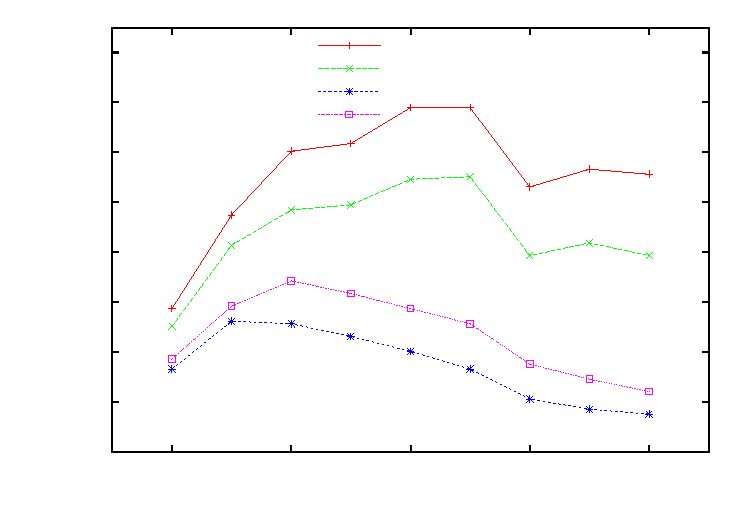
\includegraphics{messung5}}%
    \gplfronttext
  \end{picture}%
\endgroup

	\caption{...}
\end{figure}

\begin{figure}[!htb]
	\centering
	% GNUPLOT: LaTeX picture with Postscript
\begingroup
  \makeatletter
  \providecommand\color[2][]{%
    \GenericError{(gnuplot) \space\space\space\@spaces}{%
      Package color not loaded in conjunction with
      terminal option `colourtext'%
    }{See the gnuplot documentation for explanation.%
    }{Either use 'blacktext' in gnuplot or load the package
      color.sty in LaTeX.}%
    \renewcommand\color[2][]{}%
  }%
  \providecommand\includegraphics[2][]{%
    \GenericError{(gnuplot) \space\space\space\@spaces}{%
      Package graphicx or graphics not loaded%
    }{See the gnuplot documentation for explanation.%
    }{The gnuplot epslatex terminal needs graphicx.sty or graphics.sty.}%
    \renewcommand\includegraphics[2][]{}%
  }%
  \providecommand\rotatebox[2]{#2}%
  \@ifundefined{ifGPcolor}{%
    \newif\ifGPcolor
    \GPcolortrue
  }{}%
  \@ifundefined{ifGPblacktext}{%
    \newif\ifGPblacktext
    \GPblacktexttrue
  }{}%
  % define a \g@addto@macro without @ in the name:
  \let\gplgaddtomacro\g@addto@macro
  % define empty templates for all commands taking text:
  \gdef\gplbacktext{}%
  \gdef\gplfronttext{}%
  \makeatother
  \ifGPblacktext
    % no textcolor at all
    \def\colorrgb#1{}%
    \def\colorgray#1{}%
  \else
    % gray or color?
    \ifGPcolor
      \def\colorrgb#1{\color[rgb]{#1}}%
      \def\colorgray#1{\color[gray]{#1}}%
      \expandafter\def\csname LTw\endcsname{\color{white}}%
      \expandafter\def\csname LTb\endcsname{\color{black}}%
      \expandafter\def\csname LTa\endcsname{\color{black}}%
      \expandafter\def\csname LT0\endcsname{\color[rgb]{1,0,0}}%
      \expandafter\def\csname LT1\endcsname{\color[rgb]{0,1,0}}%
      \expandafter\def\csname LT2\endcsname{\color[rgb]{0,0,1}}%
      \expandafter\def\csname LT3\endcsname{\color[rgb]{1,0,1}}%
      \expandafter\def\csname LT4\endcsname{\color[rgb]{0,1,1}}%
      \expandafter\def\csname LT5\endcsname{\color[rgb]{1,1,0}}%
      \expandafter\def\csname LT6\endcsname{\color[rgb]{0,0,0}}%
      \expandafter\def\csname LT7\endcsname{\color[rgb]{1,0.3,0}}%
      \expandafter\def\csname LT8\endcsname{\color[rgb]{0.5,0.5,0.5}}%
    \else
      % gray
      \def\colorrgb#1{\color{black}}%
      \def\colorgray#1{\color[gray]{#1}}%
      \expandafter\def\csname LTw\endcsname{\color{white}}%
      \expandafter\def\csname LTb\endcsname{\color{black}}%
      \expandafter\def\csname LTa\endcsname{\color{black}}%
      \expandafter\def\csname LT0\endcsname{\color{black}}%
      \expandafter\def\csname LT1\endcsname{\color{black}}%
      \expandafter\def\csname LT2\endcsname{\color{black}}%
      \expandafter\def\csname LT3\endcsname{\color{black}}%
      \expandafter\def\csname LT4\endcsname{\color{black}}%
      \expandafter\def\csname LT5\endcsname{\color{black}}%
      \expandafter\def\csname LT6\endcsname{\color{black}}%
      \expandafter\def\csname LT7\endcsname{\color{black}}%
      \expandafter\def\csname LT8\endcsname{\color{black}}%
    \fi
  \fi
  \setlength{\unitlength}{0.0500bp}%
  \begin{picture}(7200.00,5040.00)%
    \gplgaddtomacro\gplbacktext{%
      \csname LTb\endcsname%
      \put(814,704){\makebox(0,0)[r]{\strut{} 2}}%
      \put(814,1213){\makebox(0,0)[r]{\strut{} 4}}%
      \put(814,1722){\makebox(0,0)[r]{\strut{} 6}}%
      \put(814,2231){\makebox(0,0)[r]{\strut{} 8}}%
      \put(814,2740){\makebox(0,0)[r]{\strut{} 10}}%
      \put(814,3248){\makebox(0,0)[r]{\strut{} 12}}%
      \put(814,3757){\makebox(0,0)[r]{\strut{} 14}}%
      \put(814,4266){\makebox(0,0)[r]{\strut{} 16}}%
      \put(814,4775){\makebox(0,0)[r]{\strut{} 18}}%
      \put(946,484){\makebox(0,0){\strut{} 0}}%
      \put(1783,484){\makebox(0,0){\strut{} 200}}%
      \put(2619,484){\makebox(0,0){\strut{} 400}}%
      \put(3456,484){\makebox(0,0){\strut{} 600}}%
      \put(4293,484){\makebox(0,0){\strut{} 800}}%
      \put(5130,484){\makebox(0,0){\strut{} 1000}}%
      \put(5966,484){\makebox(0,0){\strut{} 1200}}%
      \put(6803,484){\makebox(0,0){\strut{} 1400}}%
      \put(176,2739){\rotatebox{-270}{\makebox(0,0){\strut{}$\frac{\mu}{\rho}$ $[\si{\meter^2\per\kilo\gram}]$}}}%
      \put(3874,154){\makebox(0,0){\strut{}$\lambda^3~[\si{10^{-33}\meter^3}]$}}%
    }%
    \gplgaddtomacro\gplfronttext{%
      \csname LTb\endcsname%
      \put(1342,4602){\makebox(0,0)[r]{\strut{}Al}}%
      \csname LTb\endcsname%
      \put(1342,4382){\makebox(0,0)[r]{\strut{}Zn}}%
      \csname LTb\endcsname%
      \put(1342,4162){\makebox(0,0)[r]{\strut{}Sn}}%
    }%
    \gplbacktext
    \put(0,0){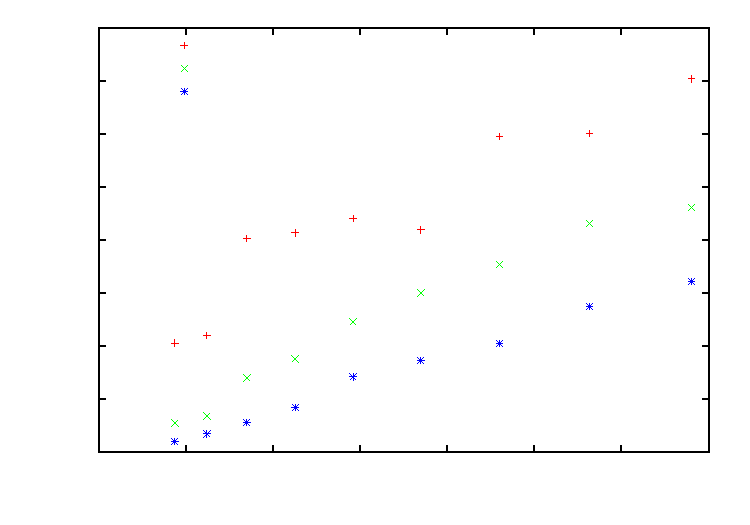
\includegraphics{messung6}}%
    \gplfronttext
  \end{picture}%
\endgroup

	\caption{...}
\end{figure}

\section{Diskussion}
\label{sec:diskussion}

\section{Anhang}

\bibliography{literatur}
\bibliographystyle{babalpha}

\end{document}
